\documentclass[../main.tex]{subfiles}
\graphicspath{{\subfix{../img/}}}


\begin{document}

\subsection{Modeling T-Type Calcium Channel} \label{sec:modeling_t_type_channel}

\subsubsection{Preface} \label{subsec:model_t_type_preface}

In conductance-based models, different authors have used different formulations for T-type $Ca^{2+}$ channels. These differences include whether activation kinetics are treated as instantaneous, the voltage ranges at which activation and inactivation gates operate, and the number of activation gates included in the model. The differences in parameters might be attributed to modelling neurons in different animal species.
% !TODO!: Citations

Furthermore, analytical and computational studies have reported that using simplified dynamics of the ion channels in the conductance based models, by assuming instantaneous kinetics, may compromize robustness of the model to parameter variations and reduce its' robustness to noise. % !TODO!: Citations

To construct biologically plausible model for \textit{Drosophila} R5 neurons which is robust to parameter variations, it would be preferable to use ion channel parameters derived directly from experimental data in \textit{Drosophila}, without simplifying the underlying kinetics.
This section presents a model for the T-type $Ca^{2+}$ ion channels based on the experimental results reported by Jeong and colleagues \parencite{jeongCaa1TFlyTtype2015}. The paper provides
information about the values for activation/inactivation variables, as well as time constants
as a functions of membrane potentials. The reported values are plotted in Figure \ref{fig:data_from_jeong}.

It is important to note a slight difference in the terminology used by Jeong and colleagues to that commonly used in modeling studies. Specifically, they report values for three types of time constants: \textbf{\textit{activation}}, \textbf{\textit{inactivation}} and \textbf{\textit{deactivation}}. The \textit{Inactivation} time constant is defined in conventional sence, as described in Section \ref{subsec:ion_channels} and corresponds to kinetics of the inactivation gate. However, both \textit{activation} and \textit{deactivation} time constants correspond to the activation gate. The term \textit{deactivation} time constant is used for measurements obtained at membrane potentials below $-50$mV, while \textit{activation} time constant refers to measurements made above $-50$mV.

This difference primarily arises from the experimental methods used to obtain the time constant values. The \textbf{\textit{activation}} time constant refers to the measurements when the membrane potential is initially held at a hyperpolarized level (where activation gates are closed), followed by a step to depolarized levels (where the activation gates open). In contrast, \textbf{\textit{deactivation}} time constant is used when the membrane potential is first held at a depolarized level and then stepped to a hyperpolarized level, causing the activation gates to close.

The fitting was performed using the \textit{SciPy} Python package. The fitted parameters, initial parameter guesses, and references to the corresponding functions are summarized in Table \ref{tab:t_type_channel_fit_summary}.

\begin{figure}[!t]
    \centering
    % First row
    \begin{subfigure}[t]{0.45\textwidth}
        \centering
        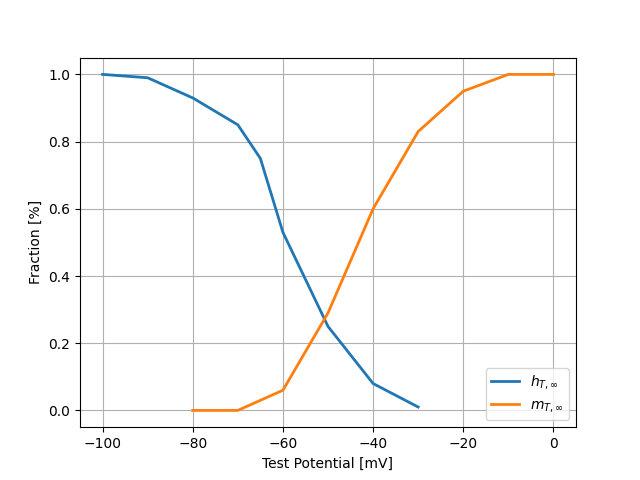
\includegraphics[width=\textwidth]{../../reports/workflow/img/t_type_calcium_channel/1_activation_and_inactivation_curves.png}
        \caption{}
    \end{subfigure}
    \hfill
    \begin{subfigure}[t]{0.45\textwidth}
        \centering
        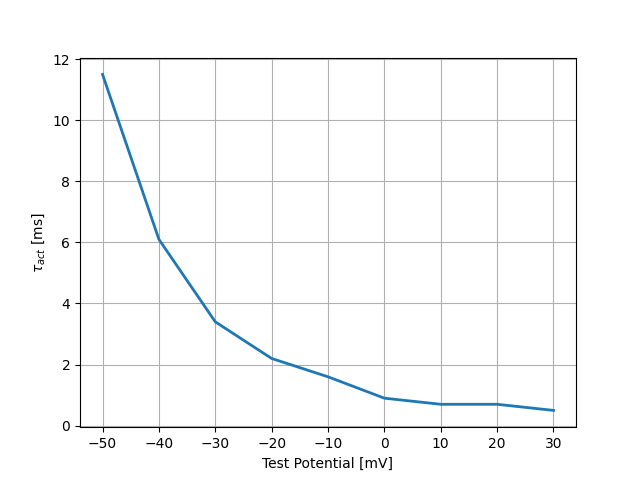
\includegraphics[width=\textwidth]{../../reports/workflow/img/t_type_calcium_channel/2_1_tau_m_jeong.png}
        \caption{}
    \end{subfigure}
    
    % Second row
    \begin{subfigure}[t]{0.45\textwidth}
        \centering
        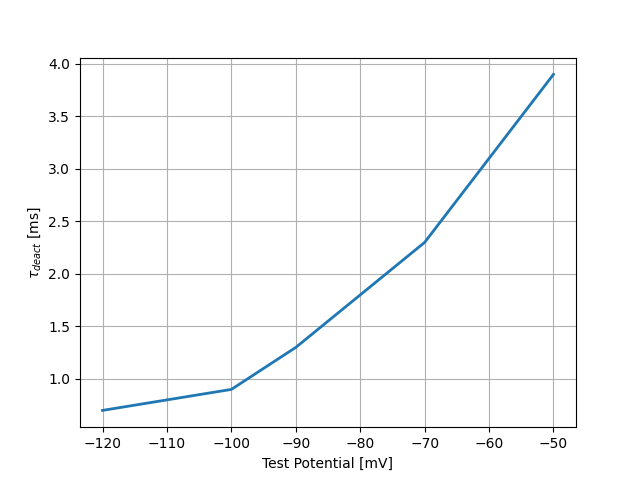
\includegraphics[width=\textwidth]{../../reports/workflow/img/t_type_calcium_channel/2_1_tau_r_jeong.png}
        \caption{}
    \end{subfigure}
    \hfill
    \begin{subfigure}[t]{0.45\textwidth}
        \centering
        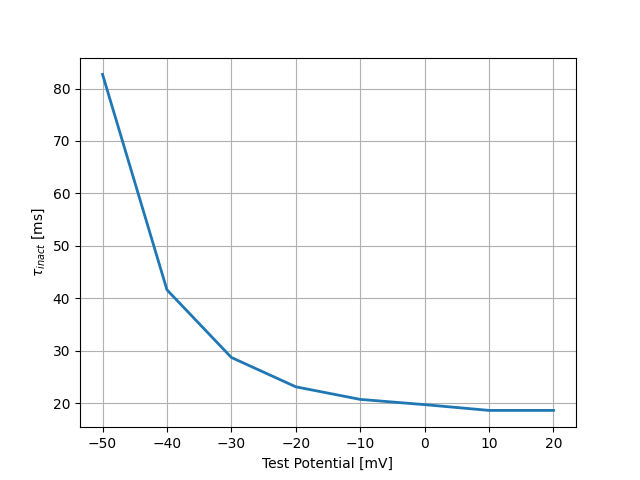
\includegraphics[width=\textwidth]{../../reports/workflow/img/t_type_calcium_channel/2_1_tau_h_jeong.png}
        \caption{}
    \end{subfigure}
    
    \caption{
        (a) Steady-state activation and inactivation functions of T-type Ca$^{2+}$ channel;
        (b) Activation, (b) deactivation and (c) inactivation as a functions of test potentials.
        Data adapted from \parencite{jeongCaa1TFlyTtype2015}. \textcolor{red}{Plots smaller, texts larger}
    }
    \label{fig:data_from_jeong}
\end{figure}


\subsubsection{Estimating gating time constants and number of activation gates}

As discussed in Section \ref{subsec:modeling_ion_channels} the current through an ion channel depends on the number of activation and inactivation gates. Depending on the experimental methodology, the steady-state curves for activation and inactivation variables, as well as corresponding time constants, may already account for the number of gates. Therefore, when fitting models to experimental data, it is important to assess whether the number of gates influences the measured parameter.

Jeong and colleagues obtanied activation time constant by two different approaches. For membrane potentials below $-50$mV the activation time constant was estimated by fitting the tail currents recorded during a voltage-setp protocol to a single exponential function (in paper referred to as deactivation time constant, \ref{fig:data_from_jeong}c). 
For membrane potentials above $-50$mV they simultaneously estimated the activation and inactivation time constants by fitting the currrent trace recorded during a step pulse protocol to a sum of two exponentials \parencite{jeongCaa1TFlyTtype2015}:
\begin{equation}\label{eq:jeong_double_exponent}
    A_1(1 - \exp{(-t/\tau_1)}) + A_2(1 - \exp{(-t/\tau_2)})
\end{equation}
where $A_1$ and $A_2$ are amplitude constants, and $\tau_1$ and $\tau_2$ are time constants. The slower time constant is generally attributed to inactivation, based on the general observation that inactivation kinetics are slower than activation kinetics \parencite{izhikevichDynamicalSystemsNeuroscience2006}.

Before estimating the functions for activation and inactivation time constants, it is important to first examine how the number of activation gates influences the measurements reported by Jeong and colleagues.

\begin{table}[!t]
    \centering
    \begin{tabular}{|c|c|c|c|c|}
        \hline
        Parameter & Fitted Value & Unit & Initial Guess & Function Reference \\
        \hline
        \hline
        $a_{m_{T,1}}$ & 0.04 & ms & & \ref{eq_model_r5_t_type_tau_m_discontinuous_below} \\
        $b_{m_{T,1}}$ & -99.6 & mV & & \ref{eq_model_r5_t_type_tau_m_discontinuous_below} \\
        $k_{m_{T,1}}$ & 36.37 & mV & & \ref{eq_model_r5_t_type_tau_m_discontinuous_below} \\
        $a_{m_{T,2}}$ & 0.56 & ms & & \ref{eq_model_r5_t_type_tau_m_discontinuous_above} \\
        $b_{m_{T,2}}$ & -13.69 & mV & & \ref{eq_model_r5_t_type_tau_m_discontinuous_above} \\
        $k_{m_{T,2}}$ & 15.2 & mV & & \ref{eq_model_r5_t_type_tau_m_discontinuous_above} \\
        $c_{\tau_{m,T}}$ & 0.467 & mV & & \ref{eq_model_r5_t_type_tau_m} \\
        $a_{h_{T}}$ & 261.5 & ms & & \ref{eq_model_r5_t_type_tau_inactivation} \\
        $b_{h_{T}}$ & -82.69 & mV & & \ref{eq_model_r5_t_type_tau_inactivation} \\
        $k_{h_{T}}$ & 7.42 & mV & & \ref{eq_model_r5_t_type_tau_inactivation} \\
        $V_{m_T,1/2}$ & -55.99 & mV & & \ref{eq:fit_jeong_gate_kinetics} \\
        $k_{m_{T}}$ & 9.32 & mV & & \ref{eq:fit_jeong_gate_kinetics} \\
        $V_{h_T,{1/2}}$ & -58.2 & mV & & \ref{eq:fit_jeong_gate_kinetics} \\
        $k_{h_{T}}$ & 7.14 & mV & & \ref{eq:fit_jeong_gate_kinetics} \\
        $V_s$ & 4.95 & mV & & \ref{eq_jeong_m_shift} \\
        $b$ & 0.45 & - & & \ref{eq_jeong_tau_scale} \\
        \hline
    \end{tabular}
    \caption[...]{
        \textbf{...}
    }
    \label{tab:t_type_channel_fit_summary}
\end{table}

%%%%%%%%%%%%%%%%%%%%%%%%%%%%%%%%%%%%%%%%%%%%%%%%%%%%%
\vspace*{0.3cm}
\noindent\textbf{Effect of number of gates on activation time constant}

To investigate how the number of gates affects the time constants estimated by fitting current trace obtaned by voltage-step protocol to Equation \ref{eq:jeong_double_exponent}, let us first consider the equation describing the current through a T-type ion channel. Assuming a single inactivation gate, using equations \ref{eq:conductance_wrt_gating_variables} and \ref{eq:ohmic_current}, the current can be expressed as:
\begin{equation}\label{eq:fitting_t_type_current}
    I_T(V,t) = \overline{g_T} m_T^p(V,t) h_T(V,t) (V - V_{Ca})
\end{equation}
where $I_T$ is the current passing through the channel, $\overline{g}_T$ is the maximal conductance, $m_T$ and $h_T$ are the activation and inactivation gating variables, and $V_{Ca}$ is the calcium reversal potential.

The voltage-step protocol begins by holding the membrane potential at a hyperpolarized value (in the current case, $-90$mV), where there inactivation gates are fully open and activation gates are closed. Next, voltage step is applied to a more depolarized potential (referred to as the \textbf{test potential}, see also Figure \ref{fig_t_type_ohmic_voltage_traces}). Thus, considering that $x_{infty}$ and $\tau_x$ ($x\in {m_T, h_t}$) depend only on voltage and not on time, using the initial conditions $m(-90,0)=0$, $h(-90,0)=1$, integration of Equation \ref{eq:fit_jeong_gate_kinetics} for each gating variable yields expressions describing their time evolution:
\begin{align*}
    m(V_f,t) = m_\infty(V_f)(1 - e^{-t/\tau_m(V_f)}) \\
    h(V_f,t) = h_\infty(V_f) + (1 - h_\infty(V_f))e^{-t/\tau_h(V_f)}
\end{align*}
where $V_f$ is the membrane potential appliied after the step in the above-mentioned protocol. Substituting these equations into Equation \ref{eq:fitting_t_type_current}, and omitting voltage dependence for simplicity (as $V_f$ is fixed during the step), one obtains:
\begin{equation*}
    I_T(t) = \overline{g_T}m^p_\infty(1 - e^{-t/\tau_m})^p \left( h_\infty + (1 - h_\infty)e^{-t/\tau_h} \right)
\end{equation*}
Expanding the expression and retaining only first-order terms in the exponentials:
\begin{align*}
    I_T(t) &\approx \overline{g_T}m^p_\infty (1 - p e^{-t/\tau_m})\left( h_\infty + (1 - h_\infty)e^{-t/\tau_h} \right) (V_f-V_{Ca})\\
    &= \overline{g_T}m^p_\infty \left(
        h_\infty + (1 - h_\infty)e^{-t/\tau_h} - p e^{-t/\tau_m} - (1 - h_\infty)p e^{-t/\tau_h}e^{-t/\tau_m}
    \right) (V_f-V_{Ca}) \\
    &\approx \overline{g_T}m^p_\infty \left(
        h_\infty + (1 - h_\infty)e^{-t/\tau_h} - p e^{-t/\tau_m}
    \right) (V_f-V_{Ca})
\end{align*}
This can be rewritten as a sum of exponentials:
\begin{equation}\label{eq:jeong_double_exponential_from_integration}
    I_T(t) = B_0 + B_1 e^{-t/\tau_m} + B_2 e^{-t/\tau_h}
\end{equation}
where $B_0=\overline{g_T}m^p_\infty h_\infty (V_f-V_{Ca})$ is a steady state component, and $B_1=\overline{g_T}m^p_\infty (1-h_\infty)$, and $B_2=\overline{g_T}m^p_\infty p$ correspond (though not necessarily in that order) to the amplitudes $A_1$ and $A_2$ in Equation \ref{eq:jeong_double_exponent}.

By comparing Equations \ref{eq:jeong_double_exponent} and \ref{eq:jeong_double_exponential_from_integration} one can see that the equation used by Jeong describes the transient component of the current trace in a first-order approximation. Moreover, within this framework, the measured time constants correspond directly to those of the individual gating variables.


%%%%%%%%%%%%%%%%%%%%%%%%%%%%%%%%%%%%%
\vspace*{0.3cm}
\noindent\textbf{Effect of number of gates on deactivation time constant}

As mentioned above, the activation time constant below membrane potentials of $50$mV was obtained by fitting the tail currents following hyperpolarizing step pulse to a single explonential function. Since activation kinetics are generally at least one magnitude faster than inactivation kinetics, the inactivation variable is generally assumed to remain constant in the time window in which the activation gates close \parencite{izhikevichDynamicalSystemsNeuroscience2006}.

As discussed in \parencite{huguenardSimulationCurrentsInvolved1992}, if an ion channel has more than one activation gates, closing any of those gates will result in reduction of the magnitude of the current. Consequently, if $p$ denotes the number of activation gates, the decay time constat of the tail current is approximately $1/p$ of the time constant associated ith a single gate. 

Therefore, time constants obtained from fitting tail currents to a single exponential should not be interpreted as the time constants of individual activation gates. Rather, if $\tau_{\text{deact}}$ is the decay time constant of current, the corresponding time constant for a single gate should be estimated as $p\tau$, where $p$ is the number of activation gates \parencite{huguenardSimulationCurrentsInvolved1992}.

%%%%%%%%%%%%%%%%%%%%%%%%%%%%%%%%%%%%%
\vspace*{0.3cm}
\noindent\textbf{Estimating number of activation gates}

As discussed above, due to specifics of the experimental procedure, the activation time constant measured by Jeong and colleagues reflecs the time constant of single acivation gate above $-50$mV. However, at potentials below $-50$mV the measured time constant scales linearly with the nubmer of activation gates. Since the authors performed both of the above-mentioned measurements at a test potential of $-50$mV, 
it is possible to estimate the number of activation gates by comparing the corresponding values of the time constants (Figures \ref{fig:data_from_jeong}b-c). When the tail currents were fitted with single exponential function, the estimated time constant at $-50$mV was $\sim 4$ms, whereas the value obtained from the second procedure at the same test potential was $\sim12$ms. Therefore, the number of activation gates in T-type $Ca^{2+}$ channels in \textit{Drosophila} is $12/4=3$.

\vspace*{0.3cm}
\noindent\textbf{Estimating activation time constant}

As discussed in Section \ref{subsec:model_t_type_preface}, both \textit{activation} and \textit{deactivation} time constants reported in the study of Jeong and colleagues refer to the \textit{activation} time constant $\tau_{m_T}$ measured above and below $-50$mV correspondingly. Initially, the time constants were fitted separately using the following exponential functions:
\begin{align}
    & \tau_{m_T}^-(V) = 3(a_{m_T,1} + \exp{[(V - b_{m_T,1})/k_{m_T,1}]}) \label{eq_model_r5_t_type_tau_m_discontinuous_below}\\
    & \tau_{m_T}^+(V) = a_{m_T,2} + \exp{[-(V - b_{m_T,2})/k_{m_T,2}]} \label{eq_model_r5_t_type_tau_m_discontinuous_above}
\end{align}
where $\tau_{m_T}^-(V)$ and $\tau_{m_T}^+(V)$ represent activation time constants below and above $-50$mV, respectively. The scaling factor of $3$ accounts for the number of activation gates, as discussed above. The resulting fits, along with the parameter values, are shown in Figure \ref{fig:data_fitted_taus_from_jeong_activation}.

\begin{figure}[!t]
    \centering
    \begin{subfigure}[t]{0.45\textwidth}
        \centering
        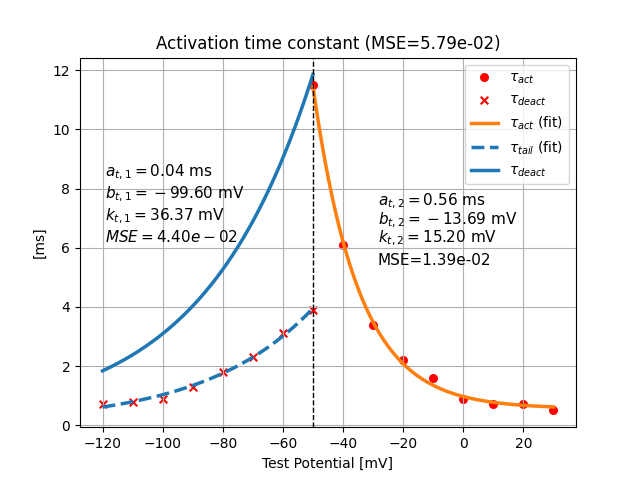
\includegraphics[width=\textwidth]{../../reports/workflow/img/t_type_calcium_channel/final_tau_activation_fit.png}
        \caption{Fitted activation and deactivation time constants using exponential functions \textcolor{red}{Change legend to tauh/3}}
        \label{fig:data_fitted_taus_from_jeong_activation}
    \end{subfigure}
    \hfill
    \begin{subfigure}[t]{0.45\textwidth}
        \centering
        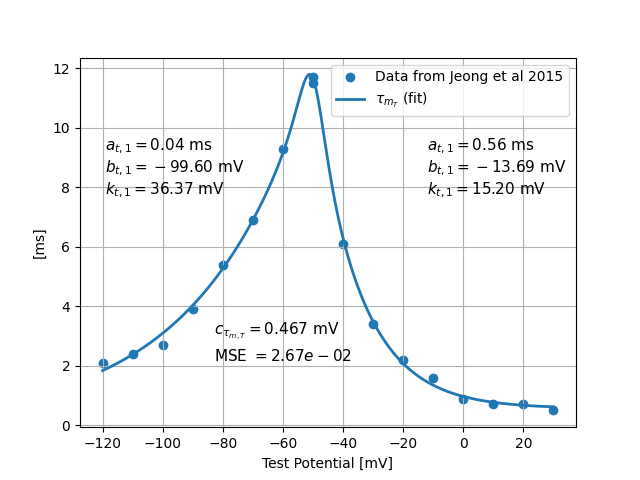
\includegraphics[width=\textwidth]{../../reports/workflow/img/t_type_calcium_channel/tau_activation_join_exponentials.png}
        \caption{Smooth transition between activation and deactivation time constants \textcolor{red}{Remove coefficient names from the plot}}
        \label{fig:data_fitted_tau_m_from_jeong_smooth_transition}
    \end{subfigure}
    
    \caption{Fitted $\tau_{m_T}$ to data from \parencite{jeongCaa1TFlyTtype2015}.}
    \label{fig:data_fitted_taus_from_jeong}
\end{figure}

To address the discontinuity at $-50$mV, the following function was introduced for smooth transition:
\begin{equation}\label{eq_model_r5_t_type_tau_m}
    \tau_{m_T}(V) = \sigma_{m_T}(V) \tau_{m_T}^-(V) + (1 - \sigma_{m_T}(V))\tau_{m_T}^+(V)
\end{equation}
where $\tau_{m_T}^-(V)$ and $\tau_{m_T}^+(V)$ are defined by Equations \ref{eq_model_r5_t_type_tau_m_discontinuous_below} and \ref{eq_model_r5_t_type_tau_m_discontinuous_above}, respectively. The weighting function $\sigma_{m_T}(V)$ was introduced to model smooth transition between the two functions and is given by:
\begin{equation}\label{eq_model_r5_t_type_channel_tau_m_sigma}
    \sigma_{m_T}(V) = \frac{1}{1 + \exp{[ c_{\tau_{m,T}} (v + 50) ]}}
\end{equation}
where $c_{\tau_{m,T}}>0$ controls the sharpness of the transition and was fitted using the combined function constructed from the the equations \ref{eq_model_r5_t_type_tau_m_discontinuous_below} and \ref{eq_model_r5_t_type_tau_m_discontinuous_above},  with the parameters in those equations fixed to the values obtained from the previous fits. The resulted smooth function, along with the fitted value of $c_{\tau_{m,T}}$ is shown in Figure \ref{fig:data_fitted_tau_m_from_jeong_smooth_transition}.

Alternative models for time constants have been proposed in the literature. One of such models, introduced by \parencite{destexheVivoVitroComputational1996}, was also implemented within the scope of this thesis. However, the model introduced in this work provided a better fit to the experimental data (\textcolor{red}{see Figure ??? - appendix}).

\vspace*{0.3cm}
\noindent\textbf{Estimating inactivation time constant}

\begin{figure}[!t]
    \centering
    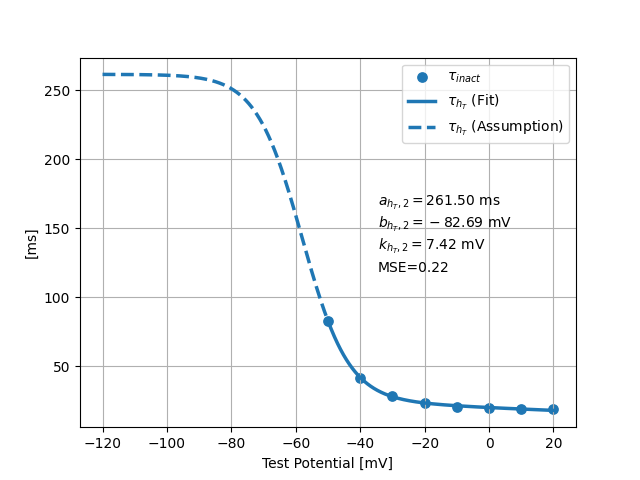
\includegraphics[width=0.45\textwidth]{../../reports/workflow/img/t_type_calcium_channel/inactivation_tau_fit_2.png}
    \caption{Fitted inactivation time constant}
    \label{fig:data_fitted_taus_from_jeong_inactivation}
\end{figure}


Inactivation time constant was modelled by the following equation proposed by \ref{wangMultipleDynamicalModes1994}:
\begin{equation}\label{eq_model_r5_t_type_tau_inactivation}
    \tau_{h_T}(V) = h_{T,\infty}(V)(a_{h_T} + \exp{[(V - b_{h_T})/k_{h_T}]})
\end{equation}
where $h_{T,\infty}(V)$ is steady state inactivation function (described below; see Equation \ref{eq:fit_jeong_gate_kinetics}). Equation \ref{eq_model_r5_t_type_tau_inactivation} was originally derived by Wang and colleagues as a simplified representation of a second-order kinetic model describing the inactivation gate of T-type channels in rat thalamocortical relay neurons \parencite{wangModelTtypeCalcium1991}. As a sidenote, higher order kinetic models account for gating mechanisms involving more than two states. For example, the model described in \parencite{wangModelTtypeCalcium1991} includes one open and two closed states for the inactivation gate of the T-type channel, rather than a simple two-state (open/closed) scheme.

Equation \ref{eq_model_r5_t_type_tau_inactivation} was fitted to the data reported in \parencite{jeongCaa1TFlyTtype2015}. The resulted fit, along with the parameters are shown in Figure \ref{fig:data_fitted_taus_from_jeong_inactivation}.

Note, that the authors of \parencite{jeongCaa1TFlyTtype2015} did not provide experimental values for inactivation time constant below $-50$mV. Although using Equation \ref{eq_model_r5_t_type_tau_inactivation} involves extrapolating the time constant into this range, any alternative choice would be equally speculative due to the absence of data.

%%%%%%%%%%%%%%%%%%%%%%%%%%%%%%%%%%%%%%%%%%%%%%%%%%%%%%%%%%%%%%%%%%%%%%%%%%%%
\subsubsection{Estimating Steady-State Activation and Inactivation Functions}

To fit the steady state activation ($m_{T,\infty}$) and inactivation ($h_{T,\infty}$) functions (Figure \ref{fig:data_from_jeong}a), the data were fitted using Boltzmann equation \parencite{huguenardSimulationCurrentsInvolved1992}:
\begin{equation} \label{eq:fit_jeong_gate_kinetics}
    x_\infty(V) = \left( \frac{1}{1 + \exp{[-(V - V_{x,1/2})/k_x]}} \right)^N \;\;\;\;\; x \in {m_T, h_T}
\end{equation}
where $V_{x,1/2}$ determines the membrane potential at which the steady-state activation/inactivation function is equal to its half-maxium, $k_x$ is corresponding slope factor,
and $N$ is a constant corresponding to the number of gates. For activation gate $N$ was set to $3$ (see discussion above), and for inactivation gate $N$ was set to $1$.
The results are shown in Figure \ref{fig:data_steady_state_from_jeong}.

\FloatBarrier


\begin{figure}[!t]
    \centering
    % First row
    \begin{subfigure}[t]{0.45\textwidth}
        \centering
        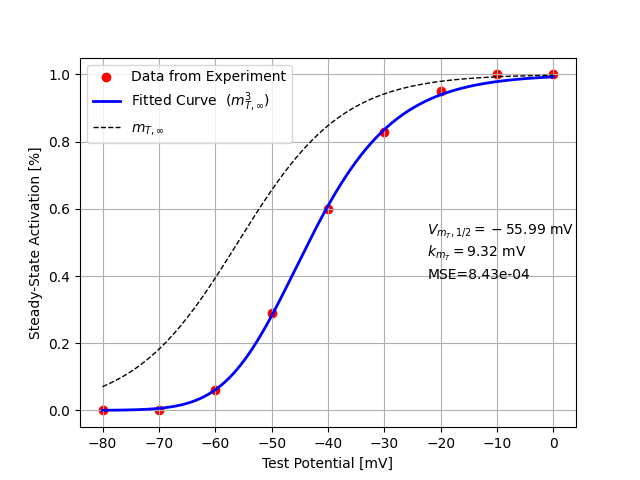
\includegraphics[width=\textwidth]{../../reports/workflow/img/t_type_calcium_channel/3_fitted_steady_state_activation.png}
    \end{subfigure}
    \hfill
    \begin{subfigure}[t]{0.45\textwidth}
        \centering
        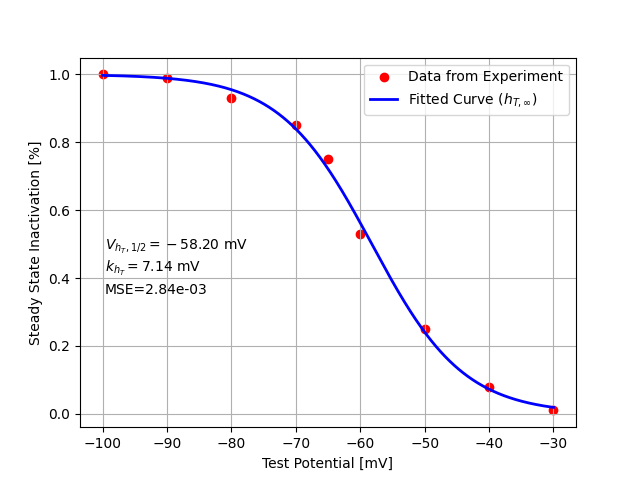
\includegraphics[width=\textwidth]{../../reports/workflow/img/t_type_calcium_channel/5_fitted_steady_state_inactivation.png}
    \end{subfigure}
    
    \caption{Fitted data to \parencite{jeongCaa1TFlyTtype2015}. \textcolor{red}{change sign of k for inactivation to match the function + A-D}}
    \label{fig:data_steady_state_from_jeong}
\end{figure}


%%%%%%%%%%%%%%%%%%%%%%%%%%%%%%%%%%%%%%%%%%%%%%%%%%%%%%%%%%%%%%%%%%%%%%%

\subsubsection{Fitting Current-Voltage Relationship}

To assess model performance, the membrane current was simulated, and the resulting transient current–voltage (I-V) relationship was compared to the experimental data reported in \textcite{jeongCaa1TFlyTtype2015} as described in Section \ref{sec:materials_and_methods}.

The current through the ion channel was first modelled using Ohm's law (see Equation \ref{eq:ohmic_current}). The reversal plotential for calcium was estimaged using Nernst equation
(see Equation \ref{eq:nernst_equation}). Intracellular and extracellular calcium concentrations were taken to be $[Ca]_i=23 nM$, and $[Ca]_o = 0.5 mM$, respectively, based on measurements in \textit{Drosophila} motor neurons \parencite{macleodFastCalciumSignals2002}.

In the Nernst equation, $R$ is the universal gas constant
($\approx 8.3145 J/K^\circ \cdot \text{Mol}$), $T$ is temperature is Kelvin (here, $273.16+25=298.16^{\circ}$), $F$ is Faraday's constant
($\approx 9.6485 \times 10^{4} C\cdot \text{mol}^{-1}$), $z$ is the valence of the ion ($z=2$ for $Ca^{2+}$). These yeilded a calcium reversal potential of $V_{Ca}\approx 128$mV. The maximal conductance was set to $0.4$ ms/cm$^2$. However, the exact value is not critical in this context, as \textcite{jeongCaa1TFlyTtype2015} reported the amplitude of the transient current in relative terms, normalized to the maximum observed value.

Figure \ref{fig_t_type_ohmic_voltage_traces} shows the test potentials applied to the model neurons, along with the simulated current trace and dynamics of the activation and inactivation variables in the case when the current was simulated via Ohmic current. Figure \ref{fig_t_type_ohmic_iv_relationship} shows corresponding transient I-V relationship.

\begin{figure}[!t]
    \centering
    % First row
    \begin{subfigure}[t]{0.45\textwidth}
        \centering
        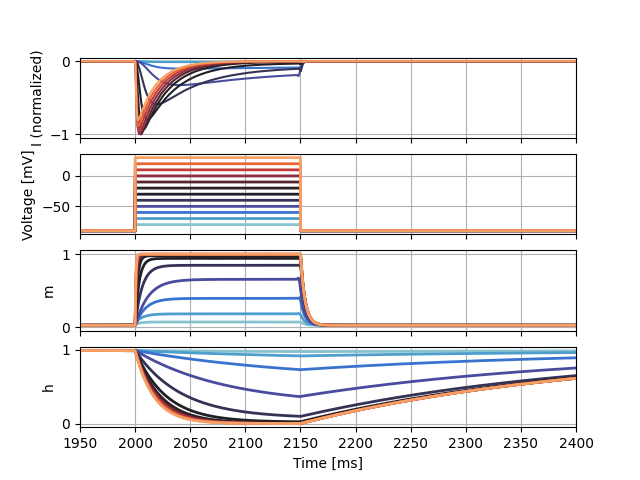
\includegraphics[width=\textwidth]{../../reports/workflow/img/t_type_calcium_channel/simulations/No Scale/Ohm's LawVoltage Step Up-Down6_voltage_traces.png}
        \caption{}
        \label{fig_t_type_ohmic_voltage_traces}
    \end{subfigure}
    \hfill
    \begin{subfigure}[t]{0.45\textwidth}
        \centering
        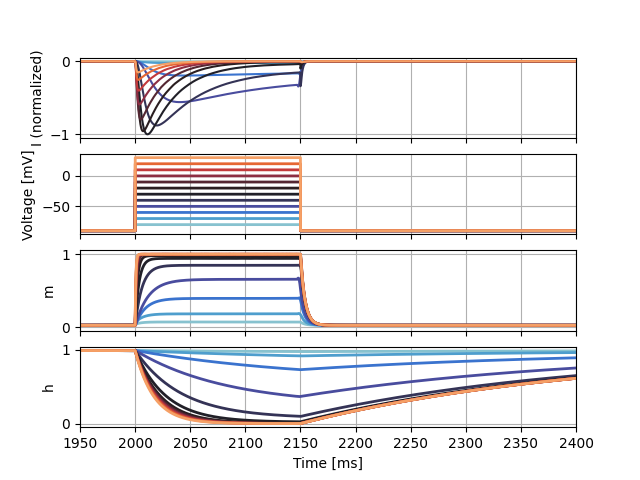
\includegraphics[width=\textwidth]{../../reports/workflow/img/t_type_calcium_channel/simulations/No Scale/Constant Field EquationVoltage Step Up-Down6_voltage_traces.png}
        \caption{}
        \label{fig_t_type_constant_field_voltage_traces}
    \end{subfigure}

    % Second row
    \begin{subfigure}[t]{0.45\textwidth}
        \centering
        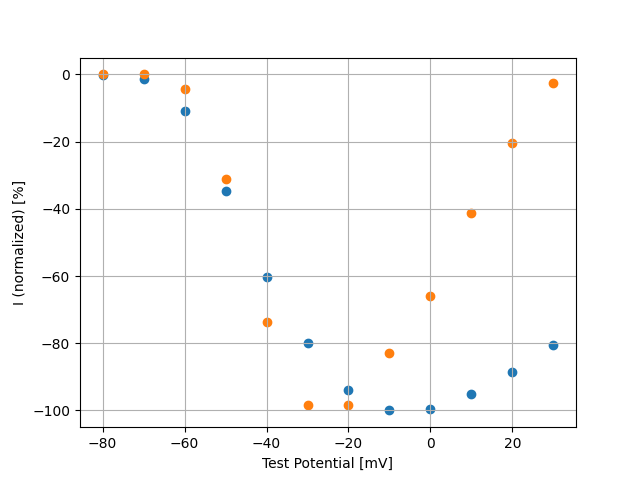
\includegraphics[width=\textwidth]{../../reports/workflow/img/t_type_calcium_channel/simulations/No Scale/Ohm's LawVoltage Step5_IV_Relationship_comparison_Jeong_2015.png}
        \caption{}
        \label{fig_t_type_ohmic_iv_relationship}
    \end{subfigure}
    \hfill
    \begin{subfigure}[t]{0.45\textwidth}
        \centering
        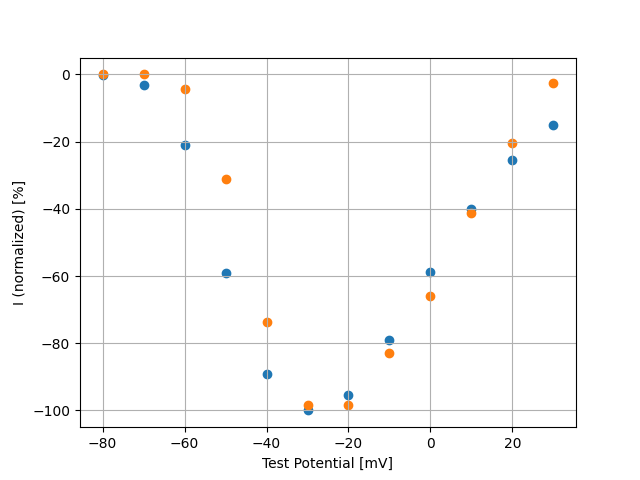
\includegraphics[width=\textwidth]{../../reports/workflow/img/t_type_calcium_channel/simulations/No Scale/Constant Field EquationVoltage Step5_IV_Relationship_comparison_Jeong_2015.png}
        \caption{}
        \label{fig_t_type_constant_field_iv_relationship}
    \end{subfigure}
    
    \caption{Ohm's low vs constant-field equation for T-Type $Ca^{2+}$ current.}
    \label{fig_t_type_voltage_step_ohmic_vs_constant_field}
\end{figure}

As shown in Figure \ref{fig_t_type_ohmic_iv_relationship}, the model failed to accurately capture the current-voltage relationship at higher test potentials. Several studies have suggested to use \gls{ghk} current equation (see Equation \ref{eq:ghk_current}) to model T-type calcium channels \parencite{huguenardSimulationCurrentsInvolved1992}. The \gls{ghk} equation explicitely models nonlinear relationship between membrane potential, ion concentations, and temperature and has been reported to yield better estimates for the T-type calcium channels. % !TODO!: cite more about ghk

\begin{figure}[!t]
    \centering
    % First row
    \begin{subfigure}[t]{0.45\textwidth}
        \centering
        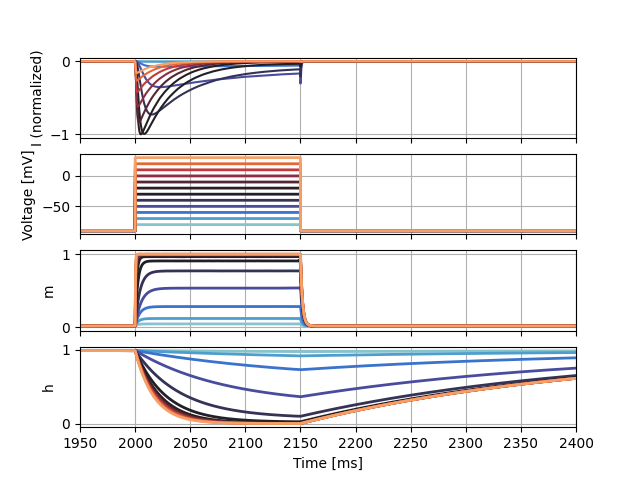
\includegraphics[width=\textwidth]{../../reports/workflow/img/t_type_calcium_channel/simulations/Scaling/Constant Field EquationVoltage Step Up-Down6_voltage_traces.png}
        \caption{}
        \label{fig_t_type_constant_field_voltage_traces_scaled}
    \end{subfigure}
    \hfill
    \begin{subfigure}[t]{0.45\textwidth}
        \centering
        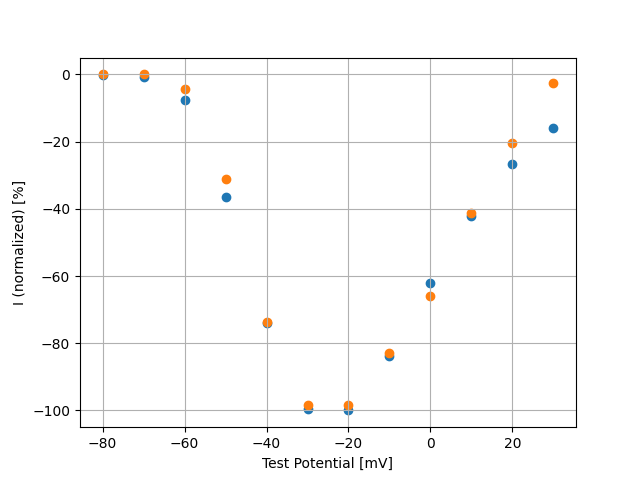
\includegraphics[width=\textwidth]{../../reports/workflow/img/t_type_calcium_channel/simulations/Scaling/Constant Field EquationVoltage Step5_IV_Relationship_comparison_Jeong_2015.png}
        \caption{}
        \label{fig_t_type_constant_field_iv_relationship_scaled}
    \end{subfigure}
    
    \caption{\textcolor{red}{Reconstructed I-V relationship after scaling and shifting activation gate time constant}}
    \label{fig_t_type_voltage_step_ohmic_vs_constant_field_scaled}
\end{figure}

All constants ($R$, $T$, $F$, $z$, $[Ca]_i$, $[Ca]_o$) were set to the same values as in the case of the Ohmic current. The maximal permeability was set to $2.47\times10^{-7}$, however, as with the Ohmic current, the exact value is not critical due to the use of relative current amplitudes in the I-V relationship.

The comparison of the simulated and experimentally obtained I-V relationships is showed in Figures \ref{fig_t_type_constant_field_voltage_traces} and \ref{fig_t_type_constant_field_iv_relationship}. Consisent with the previous reports \parencite{huguenardSimulationCurrentsInvolved1992}, modeling calcium current through the T-type channel using the \gls{ghk} current equation yeilded better estimates than the Ohmic model. However, in the case of \gls{ghk} current, the model did not accurately estimate the transient current amplitudes at more hyperpolarized test potentials.
% !TODO!: cite several in "previous reports"

There may be several factors contributing to the difference between the simulated and experimental I-V relationships. T-type $Ca^{2+}$ channels are also permeable to $Ba^{2+}$, and Jeong and colleagues used $Ba^{2+}$ recording solution to estimate steady state activation and inactivation curves.
In mammalian homologes of T-type $Ca^{2+}$ channels, it has been demonstrated that half maximal activation and inactivation potentials (i.e. the membrane potential at which $x_{\infty}=0.5$ for $x\in {m_T, h_T}$), as well as corresponding time constants, can vary depending on whether $Ca^{2+}$ or $Ba^{2+}$ is used during estimation of kinetic variables \parencite{khanPermeationGatingCaV312008}.

To test if this effect could explain the difference, a voltage shift $V_s$ was applied to the activation variable, and the corresponding time constant was scaled by $b$:
\begin{align}
    \overline{m}_{T,\infty}(V) &= m_{T,\infty}(V-V_s) \label{eq_jeong_m_shift} \\
    \overline{\tau}_{m_T}(V) &= b \tau_{m_T}(V) \label{eq_jeong_tau_scale}
\end{align}
where $m_{T,\infty}(V)$ and $\tau_{m_t}$ are governed by Equations \ref{eq:fit_jeong_gate_kinetics} and \ref{eq_model_r5_t_type_tau_m}, with corrsponding parameters given in Table \ref{tab:t_type_channel_fit_summary}. The values for $V_s$ and $b$ were fitted using the python \textit{SciPy} library to minimize the mean square error between the simulated and experimentally observed I-V relationship. The results of the fitting are shown in Figure \ref{fig_t_type_voltage_step_ohmic_vs_constant_field_scaled}. The fitted parameters were $V_s=4.95$mV and $b=0.45$. It can be seen visually, that the fit was improved in comparison to Figure \ref{fig_t_type_voltage_step_ohmic_vs_constant_field}d.

Additional fitting was performed by also shifting the inactivation steady-state function and scaling its time constant. However, this approach did not result in a substantial improvement in accuracy and is not shown here.

% \begin{itemize}
%     \item $[Ca]_{outside}$, as well as solutions used during voltage-clamp experiments
%     (calcium vs barium, as well as corresponding concentations) affects gating constants,
%     including for mammalian homologes of Drosophila T-Type Ca channels.
%     \item To my knowledge, how exactly the time constants are affected for Drosophila T-Type Ca channels
%     has not been reported.
%     \item For now: shifted steady state activation and scaled tau activation (python function curve\_fit
%     with initial guesses p0=[4, 0.5] for shift and scale correspondingly)
%     \item m(v) to m(v-4.95)
%     \item tau to tau*0.45
% \end{itemize}



% \begin{figure}[H]
%     \centering
%     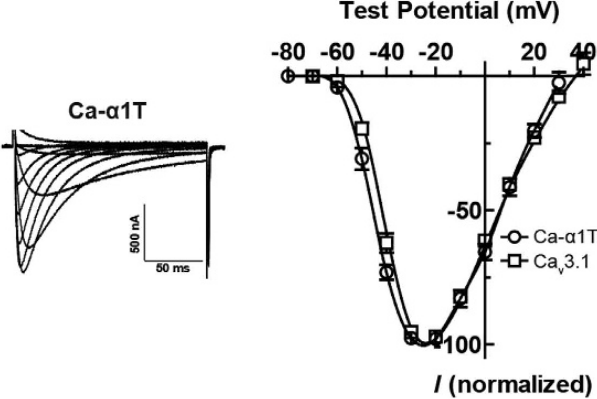
\includegraphics[width=0.45\textwidth]{../../reports/workflow/img/t_type_calcium_channel/iv_relationship_jeong_2015.png}
%     \caption{I-V relationship of T-Type $Ca^{2+}$ current in Drosophila. Adapted from \parencite{jeongCaa1TFlyTtype2015}.}
%     \label{fig:i_v_relationship_jeong}
% \end{figure}

% \begin{figure}[H]
%     \centering
%     % First row
%     \begin{subfigure}[t]{0.45\textwidth}
%         \centering
%         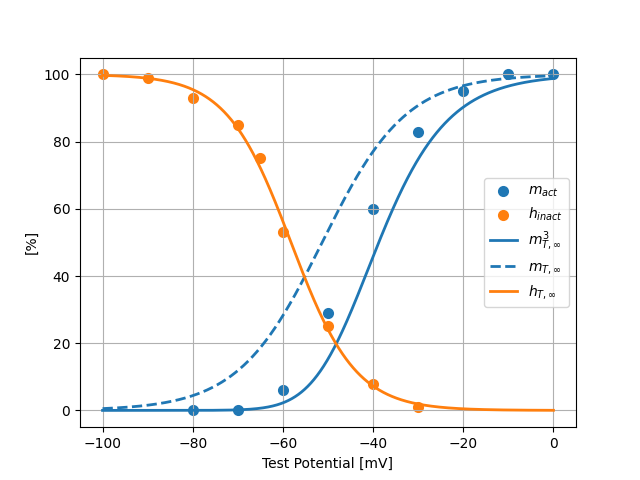
\includegraphics[width=\textwidth]{../../reports/workflow/img/t_type_calcium_channel/simulations/Scaling/Constant Field Equation1_steady_state_activation_inactivation.png}
%         \caption{}
%         \label{fig_r5_t_type_steady_state_activation_shifted}
%     \end{subfigure}
%     \hfill
%     \begin{subfigure}[t]{0.45\textwidth}
%         \centering
%         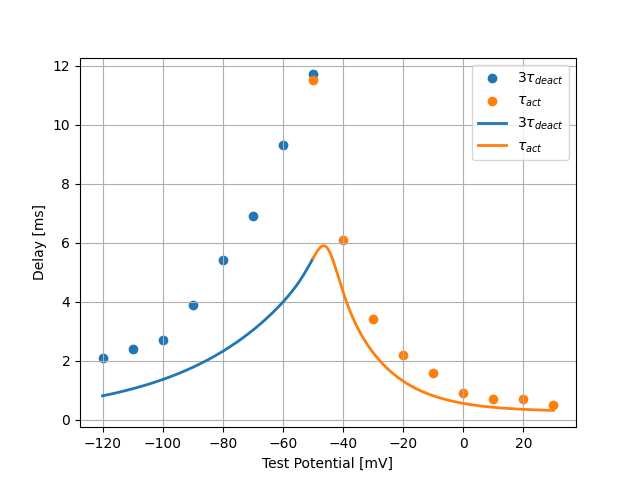
\includegraphics[width=\textwidth]{../../reports/workflow/img/t_type_calcium_channel/simulations/Scaling/Constant Field Equation2_tau_m.png}
%         \caption{}
%         \label{fig_r5_t_type_tau_activation_scaled}
%     \end{subfigure}
    
%     \caption{\textcolor{red}{Shifting and scaling time constants of activation gate}}
%     \label{fig_r5_t_type_shifting_scaling}
% \end{figure}





\end{document}